\section*{סיכום הרצאה: משוואות דיפרנציאליות חלקיות ומשוואת הגלים}

בהרצאה זו עסקנו בסיווג משוואות דיפרנציאליות חלקיות (\LR{PDEs}) מסדר שני, מעבר לצורה קנונית (\LR{Canonical Form}), ופתרון עמוק של משוואת הגלים החד-ממדית. סיימנו במבוא להפרדת משתנים במיתר סופי תוך שימוש בתורת שטורם-ליוביל.

\section{סיווג משוואות וצורה קנונית - חזרה והרחבה}

נתונה משוואה דיפרנציאלית חלקית ליניארית מסדר שני מהצורה הכללית:
$$ A u_{xx} + 2B u_{xy} + C u_{yy} = F(x, y, u, u_x, u_y) $$
סוג המשוואה נקבע על ידי הדיסקרימיננטה $\Delta = B^2 - AC$:
\begin{itemize}
    \item $\Delta > 0$: משוואה היפרבולית (\LR{Hyperbolic}) - שתי משפחות של קווים אופייניים (\LR{Characteristics}) ממשיים.
    \item $\Delta = 0$: משוואה פרבולית (\LR{Parabolic}) - משפחה אחת של קווים אופייניים.
    \item $\Delta < 0$: משוואה אליפטית (\LR{Elliptic}) - אין קווים אופייניים ממשיים (קווים מרוכבים צמודים).
\end{itemize}

\begin{examplebox}{דוגמה מסכמת: המקרה הפרבולי}
נתונה המשוואה:
$$ u_{xx} + 2u_{xy} + u_{yy} = u_y $$
\textbf{שלב 1: סיווג} \\
המקדמים הם $A=1, B=1, C=1$. הדיסקרימיננטה היא:
$$ B^2 - AC = 1^2 - 1\cdot 1 = 0 $$
לכן המשוואה פרבולית.

\textbf{שלב 2: מציאת הקווים האופייניים} \\
המשוואה לקווים האופייניים היא $\frac{dy}{dx} = \frac{B}{A} = 1$. מכאן:
$$ y = x + c \implies x - y = c $$
ישנה משפחה אחת של קווים: $x-y = \text{const}$.

\textbf{שלב 3: החלפת משתנים לצורה קנונית} \\
נבחר משתנים חדשים $\xi, \eta$. נבחר את $\xi$ לפי הקווים האופייניים ואת $\eta$ בצורה בלתי תלויה (למשל $x$ או $y$):
$$ \xi = x - y, \quad \eta = x $$
נחשב את הנגזרות החלקיות באמצעות כלל השרשרת (\LR{Chain Rule}):
$$ \frac{\partial}{\partial x} = \frac{\partial \xi}{\partial x}\partial_\xi + \frac{\partial \eta}{\partial x}\partial_\eta = \partial_\xi + \partial_\eta $$
$$ \frac{\partial}{\partial y} = \frac{\partial \xi}{\partial y}\partial_\xi + \frac{\partial \eta}{\partial y}\partial_\eta = -\partial_\xi $$
לאחר הצבת הנגזרות השנייה וצמצום איברים (ראה הרצאה קודמת לטכניקה המלאה), המשוואה הופכת ל:
$$ u_{\eta\eta} + u_\xi = 0 $$
\end{examplebox}

\begin{notebox}{הערה פיזיקלית על התוצאה}
המשוואה $u_{\eta\eta} = -u_\xi$ מזכירה משוואת דיפוזיה, אך עם סימן זמן "הפוך" (אם נתייחס ל-$\xi$ כזמן). משוואה כזו מתארת תהליך בו האנטרופיה קטנה והחומר מתרכז במקום להתפזר ("קונדנסציה"), דבר שאינו פיזיקלי באופן ספונטני, אך מעניין מתמטית.
\end{notebox}

\section{משוואת הגלים (\LR{The Wave Equation})}

המשוואה הקלאסית לתיאור גלים (כגון מיתר רוטט) היא משוואה היפרבולית:
$$ u_{tt} - c^2 u_{xx} = 0 $$
כאן $A = -c^2$, $B=0$, $C=1$. הדיסקרימיננטה היא $B^2 - AC = c^2 > 0$.

\subsection{מאפיינים וצורה קנונית}
הקווים האופייניים מתקבלים מפתרון המשוואה הריבועית $\frac{dt}{dx} = \pm \frac{1}{c}$, ומובילים לשתי משפחות של ישרים:
\begin{enumerate}
    \item $x - ct = \text{const}$ (גל נע ימינה)
    \item $x + ct = \text{const}$ (גל נע שמאלה)
\end{enumerate}

נגדיר קואורדינטות קנוניות:
$$ \xi = x + ct, \quad \eta = x - ct $$
לאחר הצבה במשוואה (ראה פירוט אלגברי בהמשך), האיברים $u_{\xi\xi}$ ו-$u_{\eta\eta}$ מצטמצמים, ונותרת המשוואה הפשוטה ביותר:
\begin{resultbox}{הצורה הקנונית של משוואת הגלים}
$$ u_{\xi\eta} = 0 $$
\end{resultbox}

פתרון משוואה זו הוא מיידי על ידי אינטגרציה כפולה:
$$ u(\xi, \eta) = f_1(\xi) + f_2(\eta) $$
ובחזרה למשתנים המקוריים, אנו מקבלים את הפתרון הכללי של משוואת הגלים:
$$ u(x,t) = f_1(x+ct) + f_2(x-ct) $$
זהו סכום של גל הנע שמאלה ($f_1$) וגל הנע ימינה ($f_2$) במהירות $c$.

\subsection{ויזואליזציה של קווים אופייניים}
\begin{center}
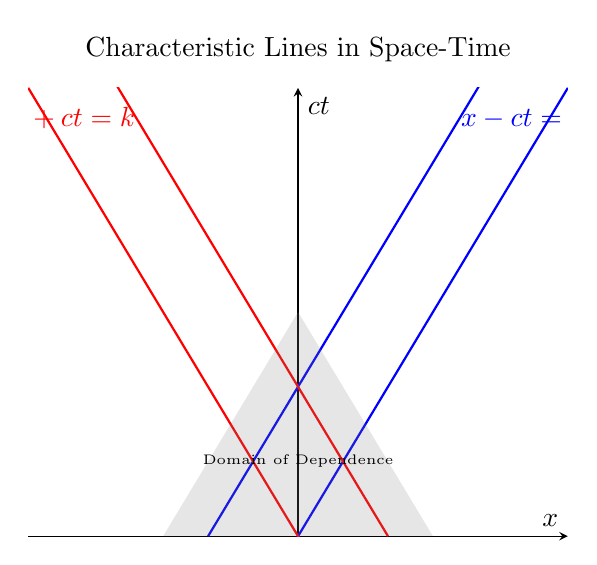
\begin{tikzpicture}
    \begin{axis}[
        axis lines=middle,
        xlabel=$x$,
        ylabel=$ct$,
        xmin=-3, xmax=3,
        ymin=0, ymax=3,
        ticks=none,
        axis line style={-stealth},
        title={\LR{Characteristic Lines in Space-Time}}
    ]
    % Characteristics x - ct = const
    \addplot[domain=-2:3, color=blue, thick] {x}; 
    \addplot[domain=-1:3, color=blue, thick] {x+1};
    \node[color=blue] at (axis cs: 2.5, 2.8) {$x-ct=k$};

    % Characteristics x + ct = const
    \addplot[domain=-3:2, color=red, thick] {-x};
    \addplot[domain=-3:1, color=red, thick] {-x+1};
    \node[color=red] at (axis cs: -2.5, 2.8) {$x+ct=k$};
    
    % Domain of dependence illustration
    \fill[gray, opacity=0.2] (0,1.5) -- (-1.5,0) -- (1.5,0) -- cycle;
    \node at (axis cs: 0, 0.5) {\tiny \LR{Domain of Dependence}};
    \end{axis}
\end{tikzpicture}
\end{center}

\section{פתרון דאלמבר (\LR{D'Alembert's Solution})}

כדי למצוא את הפונקציות $f_1, f_2$, אנו זקוקים לתנאי התחלה (בעיית קושי). נתון מיתר אינסופי עם תנאים ב-$t=0$:
\begin{enumerate}
    \item מיקום התחלתי: $u(x,0) = u_0(x)$
    \item מהירות התחלתית: $u_t(x,0) = v_0(x)$
\end{enumerate}

\subsection{פיתוח הנוסחה}
נציב $t=0$ בפתרון הכללי ונגזור אותו לפי הזמן:
1. $f_1(x) + f_2(x) = u_0(x)$
2. $c f_1'(x) - c f_2'(x) = v_0(x)$

ממשוואה (2) נבצע אינטגרציה מ-$0$ עד $x$:
$$ f_1(x) - f_2(x) = \frac{1}{c} \int_0^x v_0(s) ds + K $$
כעת יש לנו מערכת של שתי משוואות ליניאריות עבור $f_1, f_2$. נפתור אותן (חיבור וחיסור המשוואות) ונציב חזרה לפתרון הכללי $u(x,t)$. התוצאה הסופית היא:

\begin{resultbox}{נוסחת דאלמבר (\LR{D'Alembert's Formula})}
$$ u(x,t) = \frac{1}{2}\left[ u_0(x-ct) + u_0(x+ct) \right] + \frac{1}{2c} \int_{x-ct}^{x+ct} v_0(s) ds $$
\end{resultbox}

\begin{theorembox}{משמעות פיזיקלית: זרימת אינפורמציה}
ערך הפונקציה בנקודה $(x,t)$ נקבע אך ורק על ידי הנתונים ההתחלתיים בקטע $[x-ct, x+ct]$ על ציר ה-$x$.
\begin{itemize}
    \item האיבר הראשון מייצג את התפצלות ההפרעה ההתחלתית לשני גלים (חצי אמפליטודה לכל כיוון).
    \item האיבר השני מייצג את תרומת המהירות ההתחלתית שנצברת לאורך הקונוס.
\end{itemize}
\end{theorembox}

\section{בעיית המיתר הסופי והפרדת משתנים}

במציאות, מיתרים הם סופיים ($0 \le x \le L$). במקרה זה, פתרון דאלמבר אינו מספיק משום שהגלים "נתקלים" בקצוות. אנו חייבים להוסיף \textbf{תנאי שפה} (\LR{Boundary Conditions}).
הבעיה השלמה (קושי + דיריכלה/נוימן):
\begin{itemize}
    \item משוואה: $u_{tt} = c^2 u_{xx}$
    \item תנאי התחלה: $u(x,0)=u_0(x), u_t(x,0)=v_0(x)$
    \item תנאי שפה (לדוגמה, מיתר קשור): $u(0,t)=0, u(L,t)=0$
\end{itemize}

\subsection{הפרדת משתנים (\LR{Separation of Variables})}
נחפש פתרונות פרטיים מהצורה $u(x,t) = X(x)T(t)$.
נציב במשוואה:
$$ X(x)T''(t) = c^2 X''(x)T(t) \implies \frac{T''(t)}{c^2 T(t)} = \frac{X''(x)}{X(x)} = -\lambda $$
מכיוון שאגף אחד תלוי רק ב-$t$ והשני רק ב-$x$, שניהם חייבים להיות שווים לקבוע הפרדה $\lambda$.

\subsection{הקשר לתורת שטורם-ליוביל}
החלק המרחבי של הבעיה:
$$ X'' + \lambda X = 0, \quad X(0)=0, X(L)=0 $$
זוהי \textbf{בעיית שטורם-ליוביל}.
\begin{theorembox}{משפט שטורם-ליוביל (\LR{Sturm-Liouville Theorem})}
עבור אופרטור דיפרנציאלי צמוד לעצמו (\LR{Self-Adjoint}) בתחום סופי:
\begin{enumerate}
    \item הערכים העצמיים $\lambda_n$ הם ממשיים.
    \item הפונקציות העצמיות $X_n(x)$ מהוות מערכת אורתוגונלית ושלמה.
\end{enumerate}
המשמעות הפיזיקלית: ניתן לפרוס \textbf{כל} צורת מיתר $u(x,t)$ כטור אינסופי של פונקציות עצמיות (אופני תנודה או "מודים").
\end{theorembox}

בשיעור הבא נפתור את הבעיה המרחבית למציאת ה-$\lambda_n$ וה-$X_n(x)$, ולאחר מכן נפתור את החלק הזמני $T_n(t)$ כדי לקבל את הפתרון הכללי כטור.
